\documentclass[a4paper,twocolumn,12pt]{article}

\usepackage[utf8]{inputenc}
\usepackage[T1]{fontenc}
\usepackage[francais]{babel}

\usepackage{enumitem}

\usepackage[hyphens]{url}
\usepackage[colorlinks,linkcolor=blue]{hyperref}


\usepackage{fontspec}
\setmainfont{Times New Roman}

\usepackage[a4paper]{geometry}
\usepackage{graphicx}
\usepackage{wallpaper}

\title{\Huge \bfseries La consommation énergétique d'internet \\ \vspace{0.2cm}  \normalsize Séminaire EthiN2018}
%\author{Loïc Mahier \\ \small{M1 ALMA groupe 5} \and Saad Oumar Kone \\ \small{M1 ALMA groupe 5} \and Demetre Phalavandishvili \\ \small{M1 ALMA groupe 5}}
\ThisULCornerWallPaper{0.2}{picture/univNantes.png}
\date{\small{19 mars 2018}}

\begin{document}

\maketitle 

\begin{abstract}

	A une époque où internet est entré dans les mœurs ; Où nous préfèrons utiliser un moteur de recherche pour avoir une réponse plutôt que de se déplacer ou de contacter la ou les personnes pouvant répondre ; Où une grande majorité de la population a accès à internet à son domicile ou au bureau via des ordinateurs ou même en déplacement gràce à des ordiphones; A une époque enfin où l'écologie est un sujet d'ordre public, un réel problème de société suscitant de nombreuses tensions comme autour du projet Notre-Dame-des-Landes par exemple ; il est surprenant de voir que nous ne parlons pas ou du moins pas assez fort de la consommation énergétique d'internet. En effet, ''Internet représente plus de 7 \% de la consommation électrique mondiale, en croissance de 12 \% par an. Une simple recherche sur Google nécessite la même dépense énergétique que celle nécessaire à l’ébullition d’un demi litre d’eau'' \cite{1}.

\newpage

	''En France, l’infrastructure numérique consomme annuellement la production de 9 réacteurs nucléaires, soit 13 \% de l’électricité nationale" \cite{1}. Devant ces chiffres ahurissants, tentons d'y voir plus clair.

\end{abstract}

\tableofcontents

\newpage

\section{Introduction}

	Cet article a pour but de questionner sur l’un des effets négatifs d’internet, à savoir sa consommation énergétique. Cela en partant d’un point de vue général, de quelques chiffres pour aller un peu plus en profondeur et comprendre les enjeux avant d’évoquer les évolutions en cours. Ainsi nous allons commencer par dresser un constat de ce que représente la consommation énergétique actuelle d’internet, chiffres à l’appui. Nous chercherons ensuite à savoir pourquoi cette consommation est croissante et quel rôle jouent les entreprises et les usagers d’internet là dedans. Nous serons alors amenés à évoquer quelque peu la pollution qu’entraîne l’utilisation d’internet. Nous verrons après que le tableau dépeint n’est pas entièrement noir, en effet certaines entreprises ont entamé une révolution “verte”. Enfin, nous discuterons des diverses possibilités aujourd’hui en discussion pour limiter encore davantage la consommation énergétique d’internet.  \\
	
\section{La consommation énergétique actuelle d'internet}

	Tous les 4 ans, la consommation énergétique d'internet double. En ce moment, le secteur informatique occupe la troisième place dans le classement des grands consommateurs d'électricité, juste derrière la Chine et les Etats-Unis \cite{2}. Internet représente ainsi environ 7 \% de la consommation mondiale d’électricité \cite{3}. Cette énergie consommée par le domaine informatique a différentes sources, à savoir l’énergie nucléaire, le charbon, le gaz et les énergies renouvelables. En 2017 parmi cette énergie consommée par l’informatique, 40 \% l’est par les entrepôts de données et le réseau central (constitué de plusieurs réseaux connectés les uns aux autres par des lignes en fibre optique). D'après les estimations de Greenpeace (une ONGI de protection de l'environnement) pour 2020, cette consommation pourrait tripler ce qui aurait un impact important sur notre environnement \cite{3}. Selon un chercheur de l'université de Dresden, Gerhard Fettweis, la consommation énergétique du secteur informatique pourrait atteindre un seuil correspondant à la consommation mondiale de 2008 et internet pourrait devenir le plus gros consommateur d'électricité dans le monde \cite{2}. Ces constats amènent des interrogations sur la manière dont les infrastructures du monde internet sont alimentées et sur la part d'énergie renouvelable et d'énergie fossile dans la consommation énergétique d’internet. \\
	
	La figure 1 représente la répartition de la consommation énergétique entre les différentes composantes du secteur informatique : nous y trouvons les utilisateurs finaux, les entrepôts de données, les infrastructures réseaux et la fabrication des produits informatiques. Ici nous comparons la variation de la consommation énergétique de ces différentes composantes entre 2012 et 2017. Discutons tout d’abord des utilisateurs finaux. Ici nous voyons que la part dans la consommation énergétique des utilisateurs finaux a diminué, mais cela ne signifie pas qu'il y a moins d’utilisateurs finaux car le nombre d’utilisateurs augmente annuellement d'environ 7 \% \cite{4}. Même situation pour la production des produits informatiques, car la demande augmente d’année en année, il est donc surprenant qu’elle diminue. Ces diminutions sont donc liées à la hausse de la consommation des autres composantes : celles des entrepôts de données et des infrastructures réseaux. Ainsi il n’y a en fait pas de diminution de la consommation de ces composantes, il y a en réalité une augmentation importante de la consommation des deux autres composantes.

\begin{figure}[!h]	
\centerline{\includegraphics[height=10cm]{picture/diagCamenbert.png}}
\caption{Diagramme extrait de \cite{23}}
\label{diagCamenbert}
\end{figure}	

	\newpage

	La consommation des infrastructures réseaux a augmenté significativement  en 2017 par rapport à 2012 (29 \% contre 20 \%). L’un des facteurs de cette hausse est l’introduction en masse de la technologie 4G pour les ordiphones et les tablettes à travers les offres proposées par les différents opérateurs. \\

	Aussi, la hausse de la consommation énergétique des entrepôts de données s’explique par l’augmentation exponentielle des différentes applications (mobile notamment) qui ont besoin d’une connection permanente avec les serveurs présent dans les entrepôts de données. Des applications tels qu'Instagram, Snapchat, Facebook pour ne prendre que des applications de type “réseaux sociaux” en exemple, applications par ailleurs parmi les plus énergivores.
	
\section{Les responsabilitées}

	Alors que nous pourrions penser que les entreprises sont les principaux consommateurs énergétique d’internet, il se trouve que les usagers ont aussi leur part de responsabilité. Une responsabilité dont ils ne sont eux-même pas réellement conscient. En effet beaucoup de gens n’ont aucune idée du fonctionnement d’internet, de ce qu’il se passe lorsqu’il utilise un moteur de recherche ou bien du coût énergétique d’un mèl qui peut aller jusqu’à quintupler avec l’ajout d’une pièce jointe par exemple. Nous allons voir pour les entreprises et les usagers, séparément, ce qui dans leur utilisation distincte d’internet consomme de l’énergie. Nous évoquerons également les FAI (Fournisseur d'Accès Internet) qui jouent aussi un rôle dans la consommation énergétique d’internet en influençant la consommation des usagers.  
	
\subsection{Des entreprises}
	
	En ce qui concerne les entreprises, nous allons plus précisément nous attarder sur le Big Data, principal responsable de la consommation énergétique d’internet par les entreprises aujourd’hui. Devant la nécessité de stocker des données, les entreprises ont deux possibilités : elles peuvent soit passer par un prestataire, évitant ainsi les investissements initiaux élevés dans une infrastructure et les coûts conséquents de maintenance et de mise à niveau ; soit construire leur propre centre de données. \\

	Un centre des données est une usine numérique hébergeant des milliers de serveurs interconnectés entre eux traitant des milliers d'informations par seconde. Leur bon fonctionnement nécessite qu’ils soient alimentés en électricité sans interruption. Aussi, comme nous pouvons l’observer dans la vie de tous les jours, nos ordinateurs ou nos ordiphones chauffent lors d'une utilisation intense. Il en est de même pour les serveurs d’un centre de données. Ce qui impose une climatisation pour évacuer la chaleur accumulée, climatisation qui augmente encore la consommation d'électricité. Pour vous donner une idée, le coût de fonctionnement d’une climatisation parmi les dizaines présentes dans un mèl est équivalent à ce qu’il faut pour climatiser un hotel d’environs 50 chambres \cite{5}. Par ailleurs, on estime que sa climatisation représente 30 à 40 \% de la consommation énergétique d’un centre de données. \\

	La prolifération de l'informatique en nuage (internet, cloud) a entraîné la création de nombreux centres de données à travers le monde contenant des milliers de nœuds de calcul. D’après le site Data Center Map \cite{6} il y aurait actuellement 4274 centres de données dans le monde répartis dans 121 pays. Ainsi, tous ces centres de données consomment d'énormes quantités d'énergie électrique, ce qui entraîne des coûts d'exploitation élevés. Mais ces centres de données rejettent également entre autres, des émissions de dioxyde de carbone (CO2) très importantes dans l'environnement. \\

	En quelques chiffres, la consommation énergétique des centres de données représente 3 \% de l’électricité mondiale, une estimation qui pourrait monter à plus de 13 \% en 2030. En France, les centres de données consomment entre 7 et 10 \% de la production électrique nationale \cite{7}. Les émissions de dioxyde de carbone des entreprises d'internet sont actuellement estimées à 2 \% des émissions mondiales. Elles sont équivalentes aux émissions de l'industrie aéronautique (en 2007) \cite{8} et contribues de manière significative à l'effet de serre \cite{9}.

\subsection{Des FAI}

	Les fournisseur d’accès internet jouent un rôle de plus en plus important dans les émissions de gaz à effet de serre puisque la quantité d'énergie utilisée augmente de façon spectaculaire avec la croissance explosive des besoins en services. A cette demande s’ajoute l’exigence de plus en plus élevée des usagers qui veulent qu’internet soit accessible partout, à tout moment et qu’internet soit rapide. Ainsi, au fur et à mesure que les vitesses d'accès à internet augmenteront, la consommation d'énergie de l'équipement utilisé pour y accéder augmentera nécessairement. Par exemple l’alimentation d’une box et d’un boitier TV 24h sur 24 coûte à peu près 30 euros pour une consommation de 150 à 300kWs par an pour un foyer. Cela représente près de 20 \% de la production d’un réacteur nucléaire juste pour faire fonctionner les box ADSL (Asymmetric Digital Subscriber Line) en France \cite{10}. \\

	A ce coût très important des équipements, vient s’ajouter le coût lié au débit, de plus en plus élevé. Beaucoup d’entre nous aimerions avoir la fibre optique chez nous par exemple. Comme c’est déjà le cas dans les grandes villes, car les débits en campagne sont beaucoup plus faibles. Mais cette augmentation des débits augmente aussi le coût énergétique. Il permet par exemple de regarder une vidéo en haute définition, ce qui n’était pas forcément possible auparavant. Cela modifie donc le comportement des usagers. Il est d’ailleurs important de souligner que cette augmentation de débit est voulue par les usagers, les FAI n’en sont pas les uniques responsables. Comme nous le disions la responsabilité est partagée. En effet, nous souhaitons tous avoir un internet plus performant, mais au détriment, inconsciemment pour beaucoup, de l’aspect écologique.

	\newpage

	Et puisque nous avons discuté du haut débit filaire, nous pouvons aussi évoquer les nouvelles technologies sans fils tels que la 3G, la 4G ou la 5G (il s'agit là de différentes générations de norme de téléphonie mobile, d'où le G pour génération). En effet, tout ce qui est réseau sans-fil nécessite une beaucoup plus grande quantité d'énergie que le réseau filaire. Aussi, selon les estimations réalisées, le réseau 3G a besoin de 15 fois plus d'énergie que le Wifi et le réseau 4G est encore plus énergivore que ces deux derniers (environ 23 fois plus) \cite{4}. Avant l’apparition de la 4G, la consommation énergétique du réseau sans-fil était moins importante, car le débit du réseau Wifi était plus haut que celui du réseau 3G. Cela a eu pour conséquence que les utilisateurs finaux préféraient le réseaux Wifi chez eux à la 3G. L’apparition de la 4G a effacé cette frontière entre ces deux réseaux sans fil, car le débit  du réseau 4G  est beaucoup plus important que celui du réseau 3G et dans certaines conditions il est équivalent à un débit Wifi. Prochainement, l’utilisation de la 4G risque de provoquer une hyper consommation d'électricité car de plus en plus nous observons que les fabricants d'ordinateurs portables et de tablettes présentent des produits disposant d’antennes 4G. Cela se vérifie en regardant la statistique suivante qui couvre la période entre les années 2013 et 2015 \cite{4} :
	
\begin{itemize}	
	\item 2013 - 200 millions utilisateurs 4G ;
	\item 2014 - 490 millions utilisateurs 4G ;
	\item 2015 - 875 millions utilisateurs 4G ;
\end{itemize}

	\indent Nous constatons donc une tendance puisque le nombre d’utilisateurs 4G a plus que quadruplé en deux ans. Les FAI étant à l'écoute des usagers, ce chiffre risque d’augmenter dans les prochaines années, car ils proposent de plus en plus d’offres de box internet basées sur le réseau 4G pour les régions défavorisées. Ainsi, nous pouvons constater que la consommation énergétique d’internet ne dépend pas exclusivement des entreprises ou des FAI, les usagers l’influencent également.


\subsection{Des usagers}
	
	Comment mentionné plus haut, les usagers d’internet ont eux aussi leur part de responsabilité dans l'hyper consommation énergétique d’internet. Toute cette consommation est engendrée par la forte demande des usagers pour répondre à leur besoin à tous moments, comme pour envoyer un mèl par exemple ou consulter un site, faire une recherche sur un moteur de recherche, etc. Et cela depuis différentes plateformes telles qu’un ordinateur, un ordiphone ou encore une tablette. D'autant plus que nous possédons par foyer, un ordiphone par personne en général (excepté les enfants, encore que) et plusieurs ordinateurs qu’ils soient fixes ou portables. S’ajoute à cela l’apparition depuis quelques années des tablettes. Tout cet équipement est en général connecté à internet, rare sont les personnes les utilisant hors-ligne. \\

	Prenons le coût d'envoi d’un mèl sans pièce jointe, il est estimé par l’Agence de l’environnement et de la maîtrise de l’énergie (Ademe) à approximativement 5wh et celui d'un mèl avec une pièce jointe à 24 wh. Cela représente la consommation électrique pendant une heure d’une ampoule de basse consommation. A la première approche nous pourrions dire que ce n’est pas un chiffre énorme, mais si nous passons à l'échelle, en prenant en compte le nombre de mèls envoyé sans pièce jointe pendant une heure nous obtenons à la fin une quantité d'énergie correspondant au fonctionnement de 15 centrales nucléaires pendant une heure \cite{11}. \\

	Ce ne sont là que quelques chiffres pour illustrer cette consommation énergétique d’internet de la part des usagers. Ce n’est en aucun cas un constat complet du coût de notre utilisation d’internet, car chacun a des pratiques différentes et par conséquent une consommation différente. Par exemple certains vont uniquement utiliser internet pour regarder leurs mèls, là ou d’autre vont regarder un film ou jouer à des jeux vidéo, dans chaque cas la consommation sera très variable. Le fait de regarder des vidéos ou du “streaming” étant ce qui consomme le plus. \\ 

	A cela s’ajoute l’utilisation des ordiphones qui est devenu un outil indispensable de nos jours, nous l'utilisons en effet de plus en plus quotidiennement. Et cela parce que nous utilisons diverses applications pour accéder aux réseaux sociaux par exemple. Ainsi nombre d’entre nous sont connectés à internet en permanence ou presque sur leur ordiphone. Alors que d’autres ne se servent de leurs ordiphones que pour téléphoner et échanger des sms. \\

	En ce qui concerne les usagers, il y a un autre fait à étudier. En effet, la fin d'année 2017 a été marquée par la fulgurante hausse de la valeur d’une crypto-monnaie en particulier : le Bitcoin. Une crypto-monnaie est une monnaie virtuelle utilisable sur un réseau informatique décentralisé. Dans cette partie nous allons aborder la consommation énergétique du Bitcoin, qui s’obtient par un calcul de la preuve cryptographique. Autrement dit par du minage (mining en anglais) de Bitcoin, qui peut être effectué par plusieurs processeurs graphiques (GPU), interconnectés, représentant la ferme de minage. La récompense pour le calcul effectué est donnée aux mineurs qui ont résolu le défi cryptographique avant les autres. Cette récompense dépend de la puissance de calcul des cartes graphiques \cite{18}. Selon une estimation, la transaction d’un Bitcoin correspond à la consommation d’un radiateur électrique allumée pendant 4 jours, c'est-à-dire 100 kWh \cite{19}. Le nombre moyen de transaction par jour d’un bitcoin est d'environ 200 000 \cite{20}. Cela nous donne approximativement la consommation énergétique annuelle des transactions : 100 * 200 000 * 3654 = 25 * 200 000 * 365 = 1,83109 kWh \\
	
	Dans le classement de la consommation énergétique des pays, le Bitcoin consomme plus que 159 pays réunis dans le monde, ce qui représente 31 TWh \cite{18}. Mais ces chiffres ne son représentatifs que pour une seule crypto-monnaie, le Bitcion. Et à l’heure actuelle, il existe plus de 1500 crypto-monnaies différentes \cite{21}, plus ou moins populaire mais qui sont basées sur le même principe de fonctionnement que le Bitcoin. Aujourd’hui, la consommation énergétique des crypto-monnaies est très importante. En effet les fermes des mineurs peuvent être considérées comme des centres de données situés chez les usagers et tournant 24h sur 24. Pour garantir la sécurité, et les transferts liés aux crypto-monnaies partout dans le monde. Ces facteurs alourdissent la facture énergétique mondiale d’internet car la consommation énergétique des crypto-monnaies correspond à 0,10 \% de toute la production électrique mondiale \cite{22}.  \\
	
	On obtient donc au final une consommation énergétique d’internet partagée entre les entreprises d’un coté, qui mettent à notre disposition des services, souvent énergivores et les usagers de l’autre, qui disposent de ces services. Chacun a sa responsabilité et chacun a des efforts à fournir pour diminuer ce coût énergétique. Nous allons voir dans la suite que contrairement aux usagers, les entreprises essaient déjà pour certaines de rendre internet un peu plus “vert”.

\section{Les efforts déjà consentis}

	Pour qu’internet fonctionne en continu il a besoin d’une alimentation énergétique continue. Cette alimentation doit répondre aux différentes demandes au sein des centres de données : les ordinateurs centraux, les serveurs et la climatisation entre autre fonctionnant 24h sur 24. Pour diminuer cette consommation énergétique, le rôle des grandes entreprises d’internets, telles que les GAFA - Google, Apple, Facebook, Amazon par exemple est très important. D’une part car ce sont des entreprises innovantes, mais aussi parce qu’elles sont de véritables leaders et qu’elles ont le pouvoir d’inciter d’autres entreprises à en faire autant. Mais il faut aussi souligner que Amazon et Google notamment sont deux des entreprises les plus énergivores. Google à lui seul possède plus de 40 centres de données à travers le monde. C’est donc aussi une question d’image. \\ 

	Depuis 2009, Greenpeace, demande aux grands acteurs de s’engager à avoir un approvisionnement énergétique basé sur des énergies renouvelables. Cette demande a porté ses fruits, en effet nous constatons aujourd’hui que plusieurs entreprises ont commencé à s’orienter vers une diminution de leur consommation en énergies fossiles \cite{3}. \\

	Suivant un rapport fait par un militant de Greenpeace, Gary Cook, en janvier 2017, Apple et Google sont en tête de l'utilisation des énergies renouvelables et les deux sociétés continuent d’utiliser leur influence pour pousser les gouvernements ainsi que leurs fournisseurs de services publics et de l’industrie informatique à accroître l'accès à l'énergie renouvelable pour leurs opérations quotidiennes. Ainsi on constate sur la figure 2 les résultats présentés par Greenpeace dans son rapport. Résultats que nous avons dû édulcorer pour pouvoir les présenter dans cet article, en effet ils étaient beaucoup trop conséquent, nous n’avons donc conservé que quelques entreprises, les plus importantes \cite{12}.

\begin{figure}[!h]	
\centerline{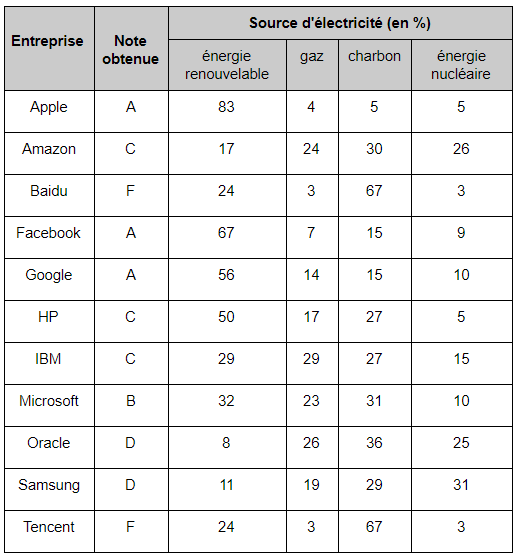
\includegraphics[height=7.5cm]{picture/tableauGreenpeace.png}}
\caption{Extrait du rapport ''Clicking clean'' de Greenpeace \cite{12}}
\label{tableauGreenpeace}
\end{figure}	
		
	Voyons plus en détail les décisions prises par quelques grands acteurs d’internet. Les géants de l’informatique ont proposé différentes approches pour diminuer l’impact sur l’environnement de leur consommation énergétique. Leurs solutions consistent notamment à utiliser des ressources naturelles telles que l'énergie solaire, le vent et même le climat de certaines régions de la planète telles que des régions aux températures très froides, pour refroidir ainsi efficacement les centres de données. Aujourd’hui Google possède un centre de données en Suède, à Hamina où la température annuelle moyenne au sud du pays est d'environ 5 degrés, et au nord de -2 degrés \cite{13,14}. Facebook a aussi suivi cette tendance en construisant l’un de leur centre de données en Suède, à Lulea \cite{15}. \\
	
	L’utilisation d’un climat froid n'est pas la seule approche des géants de l’informatique. Aux Etats-Unis, ils construisent de grandes fermes de panneaux solaires pour alimenter leurs centres de données. Cette approche est principalement utilisée par Google, Apple et Facebook. Apple possède d’ailleurs la plus grande ferme de panneau solaire au monde, juste à côté de l’un de ses centre de données. Mais ils ne suffisent pas à assurer l’autonomie énergétique du centre de données. En effet ce n’est pas suffisant car les panneaux solaires sont intermittent, la production d'électricité dépend fortement de la météo. Ainsi les pics de production d'électricité ont lieu lors des journées ensoleillées, cependant un centre de données nécessite une alimentation constante, de jours comme de nuits, qu’il fasse beau ou qu’il pleuve. \\

	Il existe encore une troisième approche qui consiste à utiliser l'énergie du vent à l'aide d'éoliennes. Ceci est répandu parmi les grandes entreprises telles que Amazon, Microsoft, Facebook et Google. Mais l'énergie du vent tout comme l'énergie solaire dépend de la météo, ce qui limite leurs utilisations par les géants d'internet \cite{16}. La solution la plus efficace est donc pour l'instant de profiter du climat propice de certaines régions.

\section{Comment rendre internet plus ''vert''}

	Comme nous l’expliquions un peu avant, grâce à des lanceurs d’alerte tel que Greenpeace et à une prise de conscience de la part de certain géant de l’informatique, nous constatons une inversion de tendance. Nous pouvions ainsi le remarquer à l’aide de la figure 2, extrait du rapport Clicking clean de Greenpeace, que ce sont principalement les entreprises américaines qui ont de l’avance en terme de part d’énergie renouvelable dans leur consommation énergétique d’internet. L’un des premiers axes à travailler pour rendre internet plus “vert” serait donc que les autres entreprises, notamment celles asiatiques y contribues. Si nous revenons encore sur la figure 2, nous voyons que Baidu et Tencent par exemple, deux des plus grosses entreprises chinoise en informatique, sont extrèmement mal notées par Greenpeace. En effet elles obtiennent la note F, qui est la plus basse possible \cite{3}. Mais c’est là peut-être un problème qui dépasse les limites d’internet. La Chine étant un énorme pollueur, il faut sans se limiter à internet, que ces régions développent davantage les énergies renouvelables. \\

	Greenpeace propose un second axe de travail orienté vers les usagers d’internet. En effet ils veulent inciter les usagers à adapter leur utilisation d’internet pour réduire leurs consommations. Cela peut se faire simplement, en évitant de regarder des vidéos en trop haute définition par exemple, ce qui diminuerait la consommation sur les bandes passantes, de même éviter de stocker des choses inutiles sur le Cloud ou de les stocker de multiples fois. “Regarder un film en basse définition permet par exemple de consommer quatre à dix fois moins d’énergie qu’un visionnage du même fichier en haute qualité graphique” \cite{3}. Ce sont de petites adaptations qui ne changeraient pas drastiquement notre quotidien et permettrait de réduire un peu la part de consommation énergétique d’internet qui incombe aux usagers. \\
	
	Si nous reprenons cette idée de duplication sur le Cloud, nous pouvons alors aussi nous questionner sur le modèle de Google qui possède chaque données sur trois centres de données différents pour palier aux pannes. Cela permet certe à Google de garantir la disponibilité de ses données auprès des usagers mais cela augmente le nombre de centre de données nécessaire et ajoute de la consommation dû aux transferts sur le réseau car il faut dupliquer les données. Il faut donc revoir nos manières d’utiliser internet voir peut-être même revoir nos exigences pour obtenir un internet moins énergivore. \\

	Et cela nous amène à un troisième et dernier axe de travail, proposé notamment par des scientifiques tel que Kris De Decker dans le Low-Tech Magazine \cite{4}. De Decker pense que le meilleur moyen de limiter la consommation énergétique d’internet serait de limiter sa vitesse, autrement dit de bloquer les débits. L’idée se défend très simplement, la hausse des débits d’internet, qu’ils soient filaires via une box internet, ou sans-fils avec la 4G et 5G entraîne nécessairement une hausse de la consommation énergétique. Mais c’est une idée qui peut faire peur, en effet comment limiter ce débit ? Est-ce les FAI qui décideront du débit ? Est-ce que celui qui sera plus aisé pourra se permettre de payer plus cher pour avoir un meilleur débit au détriment de quelqu'un moins aisé qui aura une connexion bridée ? Est-ce que les FAI feront payer plus cher les connexions aux sites énergivores tel que des sites de vidéo à la demande ? Cela nous ramène un peu à la fin de la neutralité du web qui a lieu en ce moment même au Etats-Unis. Mais cela pourra faire l'objet d'un tout autre article. \\
	
	Il y a donc de nombreux moyens de rendre internet plus “vert”, nous n’en avons cité que quelques uns. Certains sont déjà mis en place, les géants d'internet changent leurs pratiques mais cela sera beaucoup plus compliqué de faire changer les pratiques des usagers et encore plus d’aller jusqu’à réduire la qualité des services qui leur sont proposés. En effet nous sommes assez peu enclins à accepter que nos services baissent en qualité.
	
\section{Conclusion} 

	Comme vous l’aurez compris, nous l’espérons, la consommation énergétique actuelle d’internet est ahurissante et de nombreux lanceurs d’alerte préviennent que si rien n’est fait la facture écologique pourrait être très lourde. De fait un grand nombre de progrès ont été fait, notamment du côté des GAFA, qui essaient pour certaine par exemple de rendre les entrepôts de données ''vert''. Mais d’autre ne semblent pas avoir pour priorité d’améliorer la situation ou sont du moins en net retard. \\

	Aussi si les usagers n’y sont pas encore sensibilisé, il est possible qu’ils se retrouvent dans un future proche à payer la facture, avec un débit réduit ou bien que leur FAI le fasse pour eux en augmentant la facture en fonction de leur consommation. \\

	Internet a été et est toujours un réel progrès technologique mais il doit aussi devenir un progrès écologique. Cependant au delà de la prise de conscience des entreprises de l'internet, l’arrivé tant promise des IoT (Internet of Things), l’internet des objets, est assez inquiétante tant elle pourrait nuir aux efforts fournis actuellement pour contrer la pollution d’internet. En effet la multitude d’objets qui pourraient se retrouver connectée tels que les télévisions, les montres et les cafetières par exemple ne feront pas nécessairement baisser la facture écologique d’internet. \\
	
	Il est enfin utile de relativiser quelque peu cette facture énergétique. En effet il faut rappeler qu'internet même s'il est devenu énergivore permet de faire de nombreuse économies d'énergie et donc contribue d'une part à l'écologie. Que ce soit d'un point de vue administratif, nous utilisons ainsi de moins en moins de papier ou d'un point de vue des transports, nous effectuons de plus en plus d'achats sur internet et ne nous déplaçons plus en voiture. De même, nous pourrions évoquer le télétravail, de plus en plus à la mode.

\bibliographystyle{plain}
\bibliography{biblioArticleEthique}

\end{document}
